\section{The Large Hadron Collider}
%%%%%%%%%%%%%%%%%%%%%%%%%%%%%%%%%%%%%%%%%
\label{sec:LHC}

The LHC~\cite{Pettersson:291782,Bruning:782076,Bruning:815187,Benedikt:823808} at CERN, officially inaugurated on $21^\mathrm{st}$ October 2008, is the largest and most powerful hadron collider ever built. Installed in the underground tunnel which hosted the Large Electron Positron Collider (LEP)~\cite{LEPreport1,LEPreport2,Wyss:314187}, the leptonic accelerator in operation until $2^\mathrm{nd}$ November 2000, the LHC accelerator has a circular shape with a length of about 27 km and is located underground at a depth varying between 50\,m to 175\,m, straddling the Franco-Swiss border near Geneva. It is designed to collide two 7\TeV counter-circulating beams of protons resulting in a centre-of-mass energy of 14\TeV, or two beams of heavy ions, in particular lead nuclei at an energy of 2.76\TeV/nucleon in the centre-of-mass frame.

The transition from a leptonic collider to a hadronic collider entailed the following
advantages: first, it was possible to build a machine that having the same size of the previous one (and therefore accommodated in the same LEP tunnel, substantially reducing the cost and time of construction), could reach a higher energy in the centre-of-mass frame. This is due to the much lower amount of energy loss through synchrotron radiation emitted by the accelerated particles, that is proportional to the fourth power of the ratio $E/m$ between their energy and their mass. Secondly, the composite structure of protons compared to the elementary structure of electrons allows LHC to be able to access a wider energy spectrum, despite the production of many low energy particles
in a complex environment. This is a particularly important feature for a machine dedicated to the discovery of ``new'' physics.

\begin{figure}[htb]
\centering
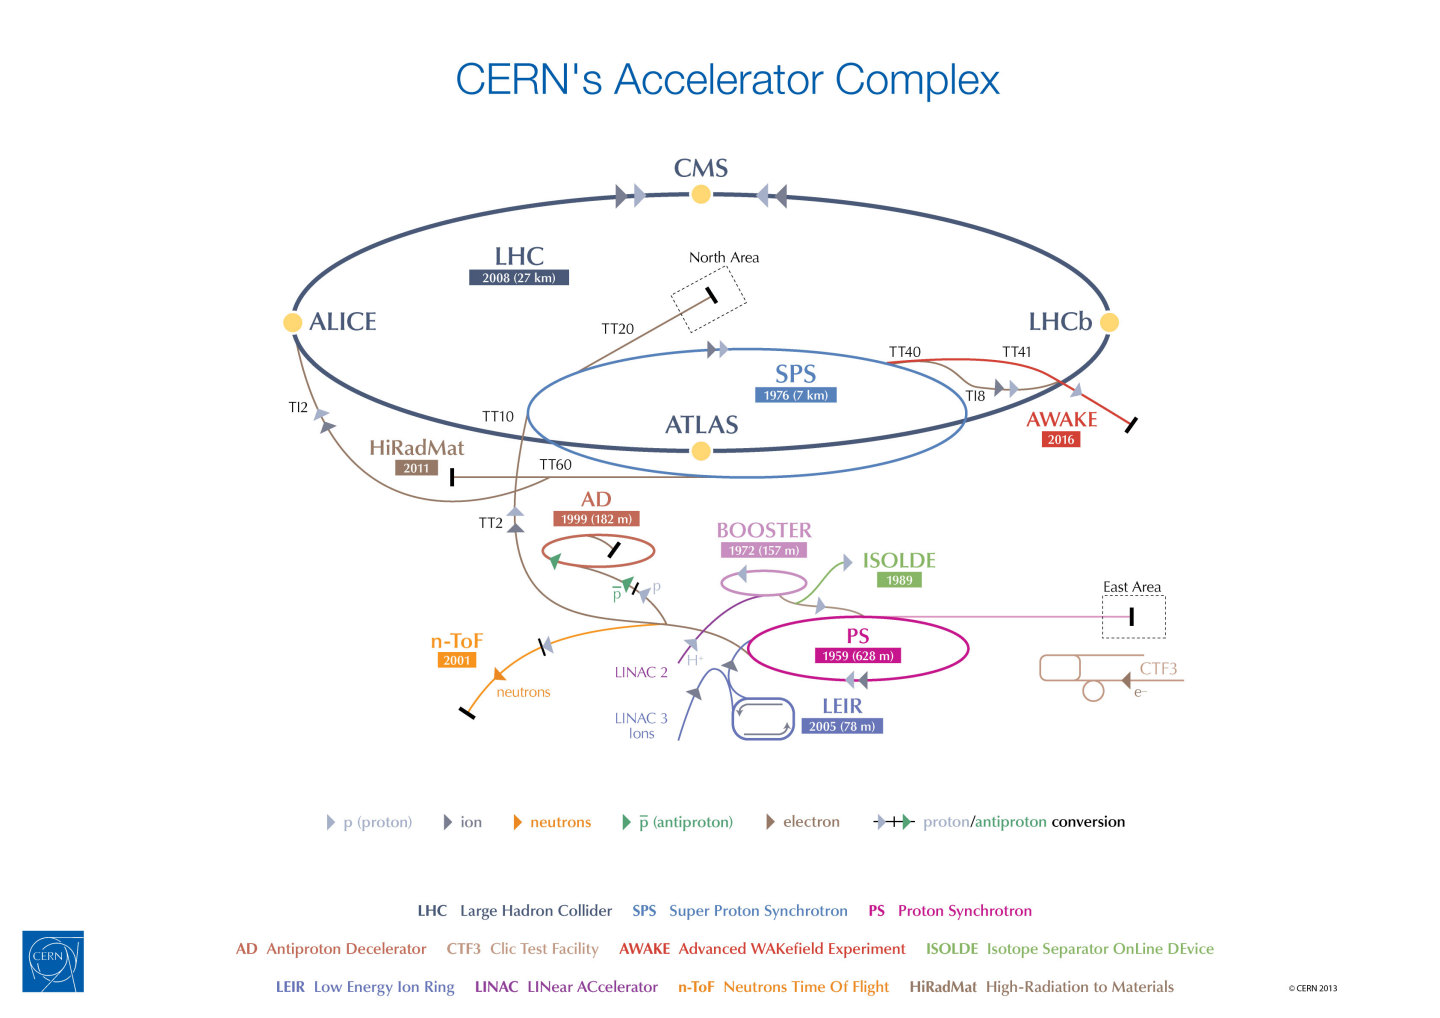
\includegraphics[width=\textwidth]{images/LHC.jpg}
\caption{Schematic description of the accelerator complex installed at CERN.}\label{fig:LHC}
\end{figure}

In Fig.~\ref{fig:LHC} a schematic description of the accelerator complex installed at CERN is shown.
The acceleration is performed in several stages~\cite{Benedikt:823808}. The protons source is a \emph{Duoplasmatron}: the protons are obtained by removing electrons from a source of hydrogen gas and then sent to the LINAC2, a 36\,m long linear accelerator which generates a pulsed beam with an energy of 50\MeV using Radio Frequency Quadrupoles (RFQ) and focusing quadrupole magnets. The beam is subsequently sent to the Proton Synchrotron Booster (PSB), a circular accelerator consisting of four superimposed synchrotron rings with a circumference of about 160\,m, which increases the proton energy up to $1.4$\GeV. Then, protons are injected into the Proton Synchrotron (PS), a single synchrotron ring with a circumference of about 600\,m where the energy is increased to 25\GeV. The sequential combination of these two synchrotrons also allows to create a series of protons bunches
interspersed by 25\,ns as required for the correct operation of LHC. The final proton injection stage is the Super Proton Synchrotron (SPS), a synchrotron with a circumference of approximately 7\,km where protons reach an energy of 450\GeV. Subsequently, protons are extracted and injected into the LHC ring via two transmission lines, to generate two beams running in opposite directions in two parallel pipes which are accelerated up to the energy of interest. In the two pipes an ultrahigh vacuum condition is maintained (about $10^{-10}$\,Torr) to avoid the spurious proton interactions with the gas remnants. At full intensity, each proton beam consists of 2808 bunches and each bunch contains around $10^{11}$ protons. The beams are squeezed for a length of about 130\,m and collide at four interaction points where the four main experiments (ALICE, ATLAS, CMS and LHCb) are placed:
\begin{itemize}
\item CMS (Compact Muon Solenoid)~\cite{Chatrchyan:2008aa} and ATLAS (A Toroidal LHC ApparatuS)~\cite{Aad:2008zzm} are two general-purpose detectors designed to investigate the largest possible spectrum of physics. In particular, they have been devoted to the detection of particles produced by Higgs boson decays and to look for any possible evidence of new physics. The use of two detectors chasing the same objectives but designed independently is crucial for a cross-check of any possible new discovery;
\item LHCb (LHC beauty)~\cite{Alves:2008zz} is an experiment primarily designed to study CP (combined charge conjugation and parity symmetry) violation in electroweak interactions and to study asymmetries between matter and antimatter through the analysis of rare decays of hadrons containing b quarks. The detector is also able to perform measurements in the forward region, at small polar angles with respect to the beam line;
\item ALICE (A Large Ion Collider Experiment)~\cite{Aamodt:2008zz} is an experiment studying heavy ions collisions, through the production of a new state of matter called quark-gluon plasma.
\end{itemize}

Two other smaller experiments are located along the circumference of the LHC accelerator, TOTEM and LHCf, which focus on particles emitted in the forward direction. TOTEM (TOTal Elastic and diffractive cross section Measurement)~\cite{Anelli:2008zza} measures the proton-proton interaction cross section and accurately monitors the luminosity of the LHC using detectors positioned at each side of the CMS interaction point. LHCf (LHC forward)~\cite{Adriani:2008zz} is made up of two detectors which sit along the LHC beamline, at a distance of 140\,m from each side of the ATLAS collision point. It makes use of neutral particles thrown in the forward direction by LHC collisions as a source to simulate the interaction of very high energy cosmic rays (between $10^{17}$\TeV and $10^{20}$\TeV) with the atmosphere in laboratory conditions.

A series of about 1200 magnetic dipoles bend the beams along the accelerator ring. They are located along the ``arc'' structures of the circumference. The ring, in fact, can be subdivided into octants, with eight curve regions (the ``arcs'') separated by rectilinear regions. In these straight regions almost 400 focusing and defocusing quadrupoles are located, which maintain the stability of the beam along the orbit, and some other small multipolar magnets (sextupoles and octupoles) are used to make additional minor corrections to the beam direction. A radio frequency acceleration system, consisting of 16 superconducting radio-frequency resonant cavities, is used to increase the proton energy by 0.5\MeV with each beam revolution. The 7\TeV per-beam-energy limit on the LHC is not determined by the electric field generated by the radiofrequency cavity but by the magnetic field necessary to maintain the protons in orbit, given the current technology for the superconducting magnets, which is about 5.4\,T on average.

One of the most important parameters of an accelerator is the instantaneous luminosity $\mathcal{L}$, which provides a measure of the rate of events one can expect given the process cross section. In fact, for a given physics process with cross section $\sigma$, producing $N$ events for unit of time, the instantaneous luminosity is defined by the following equation:
\begin{equation}
N = \sigma\mathcal{L} \quad .
\end{equation}
The LHC design luminosity is $\mathcal{L} = 10^{34} \mathrm{cm^{-2} s^{-1}}$, leading to around 1 billion proton interactions per second.

The instantaneous luminosity is a parameter which depends on the construction characteristics of the accelerator, and can be expressed by the following approximated formula:
\begin{equation}
\mathcal{L} = f\frac{n_1 n_2}{4\pi\sigma_x\sigma_y} \quad ,
\end{equation}
where $n_1$ and $n_2$ are the numbers of particles contained in the two bunches colliding at a frequency $f$, while $\sigma_x$ and $\sigma_y$ are the beam sizes in the transverse plane. At LHC, the bunches collide with $f=40$\,MHz and the transverse size of the beam can be squeezed down to around $15$\,\micron.
The integrated luminosity $L$ is defined as the time integral of the instantaneous luminosity:
\begin{equation}
L = \int \mathcal{L} dt \quad .
\end{equation}
The main parameters of the LHC machine are listed in Table~\ref{tab:LHCparams}.

\begin{table}[htb]
\caption{LHC technical parameters for proton-proton collisions: nominal, 2012 and present values are shown.}\label{tab:LHCparams}
\centering
\begin{tabular}{lc}
\toprule
{\bfseries Parameter} & {\bfseries Value}\\
\midrule
Maximum dipole magnetic field & 8.33\,T \\
Dipole operating temperature & 1.9\,K \\
\midrule
Beam energy at injection & 450\GeV \\
Beam energy at collision (nominal) & 7\TeV \\
Beam energy at collision (2012) & 4\TeV \\
Beam energy at collision (2015--2016) & 6.5\TeV \\
\midrule
Maximum instantaneous luminosity (nominal) & $10^{34}\,\mathrm{cm^{-2}s^{-1}}$ \\
Maximum instantaneous luminosity (2012) & $7.7\cdot10^{33}\,\mathrm{cm^{-2}s^{-1}}$ \\
Maximum instantaneous luminosity (2015--2016) & $1.2\cdot10^{34}\,\mathrm{cm^{-2}s^{-1}}$ \\
\midrule
Number of bunches per proton beam (nominal) & 2808 \\
Number of bunches per proton beam (2012) & 1380 \\
Number of bunches per proton beam (2015--2016) & 2220 \\
Maximum number of protons per bunch & $1.69\cdot10^{11}$ \\
\midrule
%Bunch separation in time (nominal) & 25\,\ns \\ 
%Bunch separation in time (2012) & 50\,\ns \\ 
%Bunch separation in time (2015--2016) & 25\,\ns \\
Bunch collision frequency (nominal) & 40\,MHz \\ 
Bunch collision frequency (2012) & 20\,MHz \\ 
Bunch collision frequency (2015--2016) & 40\,MHz \\
\midrule
Energy loss per turn at 14\TeV & 7\,keV \\
\bottomrule
\end{tabular}
\end{table}

The LHC started to be operative in September 2008 but, due to a faulty interconnection between two magnets that caused an explosive helium leakage in the tunnel, the operation was stopped and restarted in March 2010. During 2010 and 2011 LHC ran successfully and provided proton-proton collisions at a centre-of-mass energy of 7\TeV, delivering a total integrated luminosity of about 6.1\ifb. The encouraging results in the Higgs boson search provided by the ATLAS and CMS Collaborations led to the decision of extending the data taking period to the end of 2012, and to increase the centre-of-mass energy up to 8\TeV. During 2012, LHC delivered to the experiments an integrated luminosity of 23.3\ifb. After the first long shutdown (LS1), a two years period started in the early 2013 where the LHC operation stopped for maintenance and upgrade, the LHC started again delivering proton-proton collisions on $3^\mathrm{rd}$ June 2015, at the new record centre-of-mass energy of 13\TeV. During the 2015 the LHC delivered an integrated luminosity of 4.2\ifb. Nowadays, LHC is still colliding bunches of protons at $\sqrt{s}=13$\TeV, reaching unprecedented instantaneous luminosities and delivering a total integrated luminosity of 41.1\ifb in 2016. The cumulative delivered luminosity versus time for the different LHC data taking periods is shown in Fig.~\ref{fig:LHClumi}.

\begin{figure}[htb]
\centering
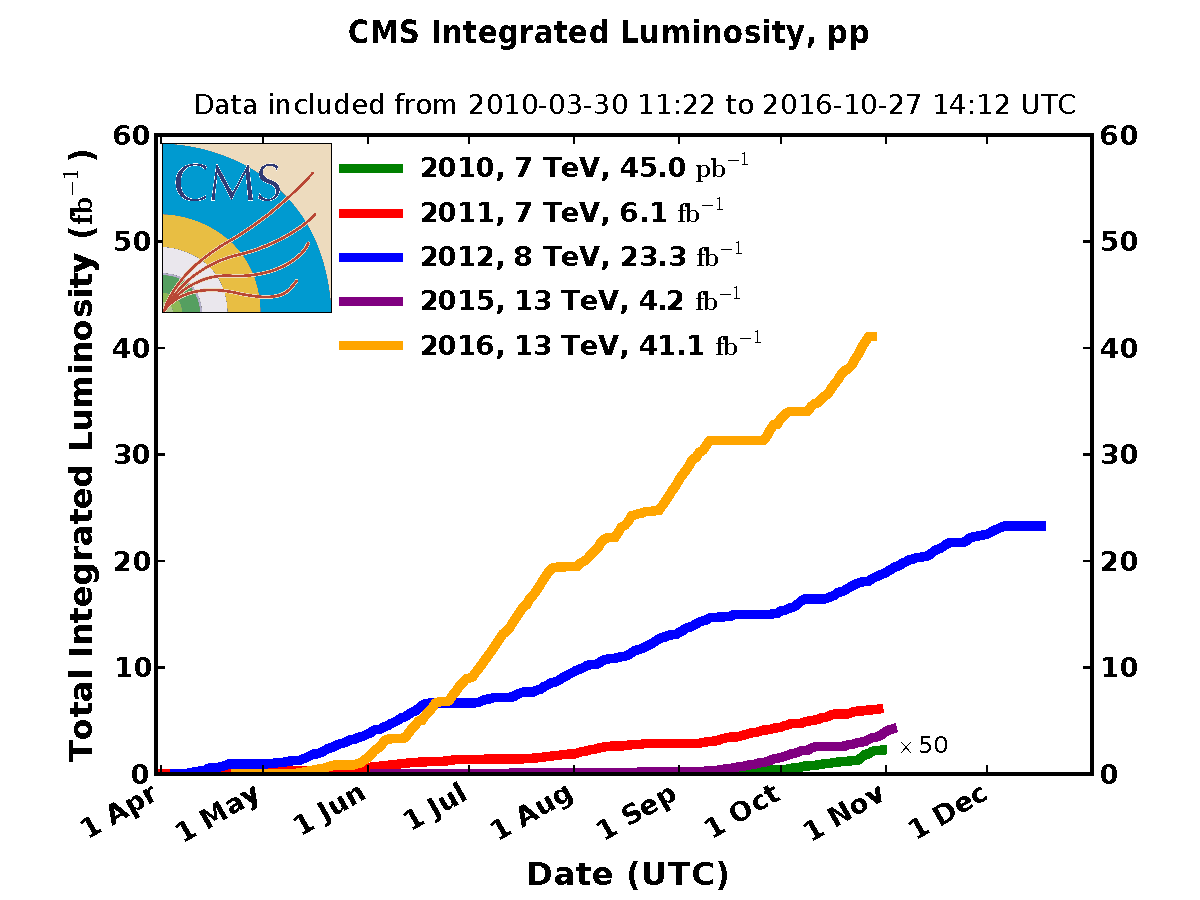
\includegraphics[width=0.7\textwidth]{images/LHClumi.pdf}
\caption{Cumulative luminosity versus day delivered to CMS during proton-proton collisions.}\label{fig:LHClumi}
\end{figure}

As the instantaneous luminosity increases, the probability of multiple proton-proton interactions to occur in a single bunch crossing grows higher as well. In this instance, the main goal is the identification and reconstruction of a single primary collision where the physics event of interest occurs among the background of the additional proton-proton interactions. Such backgrounds are due to processes occurring with very high probability, like the production of low-\pt jets. These additional collisions are known as pile-up. During the LHC current run the average number of pile-up events is 23, with some events exhibiting over 45 pile-up collisions. Two different types of pile-up may be identified: the \emph{in-time} pile-up, in which the additional collisions occur in the same bunch-crossing as the collision of interest and \emph{out-of-time} pile-up, in which the additional proton-proton collisions occur in the bunch-crossings just before or after the one containing the collision of interest.










